\chap{Techniken für den Einsatz der Schieberegler}\label{a.tech}

\sect{Einstellen der Schieberegler in den Motorblöcken}

Es ist schwierig, die Schieberegler präzise einzustellen, so dass zum Beispiel beide Motoren mit der gleichen Geschwindigkeit laufen. Wir können Präzision erhöhen, wenn wir die Übersetzung der VPL-Ereignis-Aktions-Paare in ein textbasiertes AESL-Programm  verwenden.

\trickbox{Wenn man die Schieberegler im Motorblock verschiebt, stellt man eine Sprunghafte Veränderung der Geschwindigkeit fest (\p{motor.X.target}); es handelt sich um 50er Schritte im Bereich von $-$500 to 500. Wenn man vorsichtig schiebt (oder die Cursor-Tasten verwendet) kann man jenden dieser Werte eingeben.}

Die nachfolgende \Cref{fig.textcode} zeigt das Programm aus \cref{fig.likes-hates} (wo das Haustier Sie mag und Ihnen folgt), sowie rechts die textbasierte Übersetzung des Programms. Dieser Text wird automatisch verändert, wenn man die Schieberegler betätigt.  

\begin{figure}[hbt]
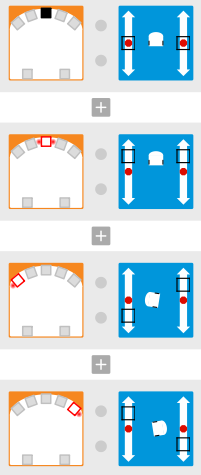
\includegraphics[width=0.3\textwidth]{likes}
\hfill
\begin{minipage}[b]{0.55\textwidth}
\begin{footnotesize}
\begin{verbatim}
onevent prox
    if prox.horizontal[2] < 1000 then
        motor.left.target = 0
        motor.right.target = 0
    end
    if prox.horizontal[2] > 2000 then
        motor.left.target = 300
        motor.right.target = 300
    end
    if prox.horizontal[0] > 2000 then
        motor.left.target = -300
        motor.right.target = 300
    end
    if prox.horizontal[4] > 2000 then
        motor.left.target = 300
        motor.right.target = -300
    end
\end{verbatim}
\end{footnotesize}
\vspace*{8ex}
\end{minipage}
\caption{Ein VPL-Programm mit dem dazugehörenden Text-Programm.}
\label{fig.textcode}
\end{figure}

\p{onevent prox} bedeutet: wann immer die Distanzsensoren ausgewertet werden (Distanzsensoren englisch \emph{proximity} sensors, abgekürzt \emph{prox}), werden die nachfolgenden Befehle bis zur Zeile \p{end} ausgeführt. Die Auswertung erfolgt 10 Mal pro Sekunde. 

Wenn das Ereignis der Auswertung eintritt, werden die Werte der Sensoren abgefragt und mit einer Selektion ausgewertet. Der Sensor mit der Nummer 2 (vorne in der Mitte) wird als erster untersucht: \p{prox.horizontal[2]}. Falls dieser Wert unter 1000 liegt, wird die Geschwindigkeit auf 0 gesetzt mit folgenden Befehlen: 

\begin{footnotesize}
\begin{verbatim}
motor.left.target  = 0
motor.right.target = 0
\end{verbatim}
\end{footnotesize}

Jeder Block \verb+if ... then ... end+ testet einen Sensor und startet die dazu passende Befehlsfolge, falls der Test zutreffend ist. Das Programm folgt dem folgenden Algorithmus: 

\begin{enumerate}[start=0,noitemsep,nosep]
\item Teste, ob nichts vor dem Roboter ist; falls dies zutrifft, hält er an.
\item Teste, ob etwas vor dem Roboter ist; falls dies zutrifft, fährt er voraus.
\item Teste, ob etwas links vor dem Roboter ist; falls dies zutrifft, dreht er sich nach links.
\item Teste, ob etwas rechts vor dem Roboter ist; falls dies zutrifft, dreht er sich nach rechts.
\end{enumerate}

Sobald die Sensoren gelesen wurden und die passende Befehlsfolge gestartet wurde, wartet das Programm auf das nächste \p{prox}-Ereignis, um die Tests erneut zu starten.  Dies wiederholt sich so lange, bis das Programm angehalten wird. 

\sect{Einstellen der Dauer des Timers}

\trickbox{Die Dauer des Timers im Aktions-Block vom Vielfachen von Viertelsekunden (250 ms) bis zu vier Sekunden eingestellt werden.}


\sect{Sensor-Ereignis-Blöcke im Fortgeschrittenen-Modus}

Dieser Abschnitt beschreibt Funktionen der Sensor-Ereignis-Blöcke, die im Fortgeschrittenen-Modus verfügbar sind. 

\subsection*{Einstellen der Schwellenwerte der Sensoren}

Im Standard-Modus sind die Schwellenwerte der Sensoren nicht veränderbar. Für die horizontalen Distanz-Sensoren bedeutet ein Wert oberhalb von 2000, dass viel Licht reflektiert wird und dass das Ereignis eintritt, falls das entsprechende Quadrat weiss ist. Ein Wert von unter 1000 bedeutet hingegen, dass zu wenig Licht reflektiert wird und ein Ereignis eintritt, wenn das entsprechende Quadrat schwarz ist. Für die unteren Sensoren liegen die Werte bei 450 und 400.

Im Fortgeschrittenen-Modus können die Schwellenwerte festgelegt werden. Mit dem oberen Schieber stellt man den Schwellenwert für ein weisses Ereignis ein und mit dem unteren Schieber die Schwelle, unterhalb derer ein schwarzes Ereignis eintritt: \label{p.proximity-sensitivity}

\begin{center}
\begin{tabular}{c@{\hspace{.1\textwidth}}c}
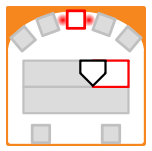
\includegraphics[width=.15\textwidth,keepaspectratio=true]{set-red}
&
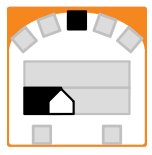
\includegraphics[width=.15\textwidth,keepaspectratio=true]{set-black}
\end{tabular}
\end{center}

\Cref{fig.follow-line-adv} zeigt das Linien-Folgen-Programm (vgl. \cref{fig.follow-line-all}) im Fortgeschrittenen-Modus. Die Schieberegler wurden so eingestellt, dass der Schwellwert sehr tief ist: 100 für den unteren und den oberen Grenzwert.

\begin{figure}
\subfigure[Roboter starten und stoppen]%
{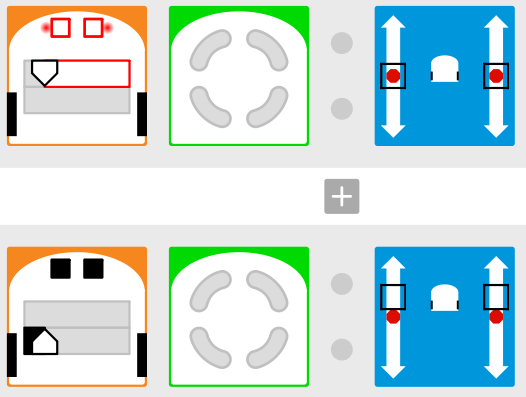
\includegraphics[width=0.45\textwidth]{line-forward-adv}}
\hfill
\subfigure[Korrektur der Abweichung]%
{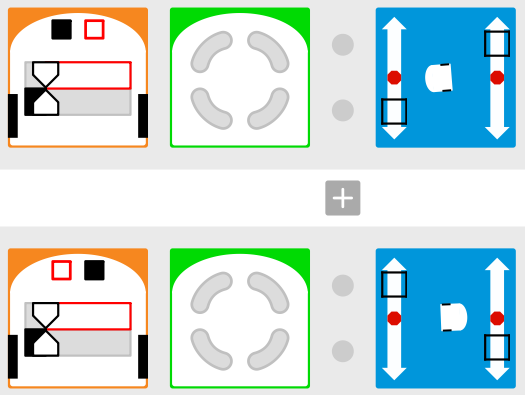
\includegraphics[width=0.45\textwidth]{line-controller-adv}}
\caption{Ein Programm zum Folgen einer Linie}
\label{fig.follow-line-adv}
\end{figure}

\subsection*{Mehrere Sensoren}

Wenn mehrere Sensoren untersucht werden, teilen sie sich die Einstellungen der Schwellwerte:
\begin{center}
\begin{tabular}{c@{\hspace{.1\textwidth}}c}
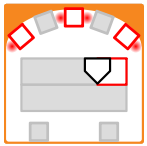
\includegraphics[width=.15\textwidth,keepaspectratio=true]{set-same}
&
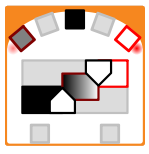
\includegraphics[width=.15\textwidth,keepaspectratio=true]{set-all}
\end{tabular}
\end{center}

\subsection*{Ereignisse für Werte zwischen Grenzwerten}

Im Fortgeschrittenen-Modus gibt es einen zusätzliches Zustand: das Quadrat kann dunkelgrau sein: \gr{set-gray}{.15}
In diesem Zustand tritt ein Ereignis ein, wenn der Wert, der gemessen wurde, zwischen dem oberen und unteren Grenzwert liegt. Der obere Grenzwert wird mit dem oberen Regler festgelegt, der unter mit dem unteren. 
